\documentclass[a4paper,10pt]{report}
\usepackage[latin1]{inputenc}
\usepackage{amsmath}
\usepackage{amsmath,bm}
\usepackage{amsthm}
\usepackage{mathtools}
\usepackage{amsfonts}
\usepackage{amssymb}
\usepackage{graphicx}
\usepackage{array}
\usepackage{booktabs}
\usepackage{hyperref}
\usepackage{multicol}
\usepackage{makecell}
\usepackage[margin=0.5in]{geometry}
\usepackage[framemethod=tikz]{mdframed}
\newcommand{\myvec}[1]{\ensuremath{\begin{pmatrix}#1\end{pmatrix}}}
\let\vec\mathbf
\newcommand{\mydet}[1]{\ensuremath{\begin{vmatrix}#1\end{vmatrix}}}
\providecommand{\mbf}{\mathbf}
\providecommand{\pr}[1]{\ensuremath{\Pr\left(#1\right)}}
\providecommand{\qfunc}[1]{\ensuremath{Q\left(#1\right)}}
\providecommand{\sbrak}[1]{\ensuremath{{}\left[#1\right]}}
\providecommand{\lsbrak}[1]{\ensuremath{{}\left[#1\right.}}
\providecommand{\rsbrak}[1]{\ensuremath{{}\left.#1\right]}}
\providecommand{\brak}[1]{\ensuremath{\left(#1\right)}}
\providecommand{\lbrak}[1]{\ensuremath{\left(#1\right.}}
\providecommand{\rbrak}[1]{\ensuremath{\left.#1\right)}}
\providecommand{\cbrak}[1]{\ensuremath{\left\{#1\right\}}}
\providecommand{\lcbrak}[1]{\ensuremath{\left\{#1\right.}}
\providecommand{\rcbrak}[1]{\ensuremath{\left.#1\right\}}}
\begin{document}\raggedright{
\includegraphics[scale=0.03]{logo.png}}\hspace{12.425cm}\raggedleft FWC22037\vspace{2mm}\\
\centering\Large\textbf{ASSIGNMENT-MATRICES}\vspace{5mm}
\begin{multicols}{2}
\centering \large\textsc{C}\footnotesize\textsc{ONTENTS}\vspace{5mm}\\
\raggedright\large\textbf{1\hspace{1cm}Problem}\hspace{5.2cm}1\vspace{5mm}\\
\raggedright\large\textbf{2\hspace{1cm}Solution}\hspace{5.25cm}1\vspace{5mm}\\
\raggedright\large\textbf{3\hspace{1cm}Construction}\hspace{4.25cm}2\vspace{5mm}\\
\centering \large\textsc{1  P}\footnotesize\textsc{ROBLEM}\vspace{5mm}\\
	\raggedright\large{Find the equation of the tangent and the normal to the hyperbola} $$ \frac{x^{2}}{a^{2}} - \frac{y^{2}}{b^{2}} = 1 $$ at the point $(x_0,y_0)$.\vspace{5mm}\\
\centering \large\textsc{2  S}\footnotesize\textsc{OLUTION}\vspace{5mm}\\
\raggedright\large{1. The give hyperbola equation can be represented as  }
\begin{gather*}
\vec{x}^{\top}\vec{V}\vec{x} + 2\vec{u}^{\top}\vec{x}+f = 0 \\
\vec{x}^{\top}\myvec{\frac{1}{a^{2}} & 1 \\ 0 & \frac{-1}{b^{2}}}\vec{x} + 2\myvec{0&0}\vec{x} -1 = 0 \\
\end{gather*} \vspace{2mm}\\
2.Equation of tangent is
\begin{gather*}
\vec{(Vq+u)}^{\top}\vec{x} + \vec{u}^{\top}\vec{q} + f =0\\
\sbrak{\myvec{\frac{1}{a^{2}}& 0 \\ 0  & \frac{-1}{b^{2}}}\myvec{x_0 & y_0} + \myvec{0 \\ 0}}^{\top}\\\vec{x} + \myvec{0 & 0}q - 1 = 0\\
\end{gather*}
\begin{align}
\myvec{\frac{x_0}{a^{2}} & \frac{-y_0}{b^{2}}}\vec{x} = 1 
\end{align}
Therefore equation of tangent is \begin{align}
 \left( \frac{x_0}{a^{2}} \right)x - \left(\frac{y_0}{b^{2}}\right)y = 1 
\end{align}
3. Equation of normal is 
\begin{gather}
\vec{m}^{\top}(\vec{x-p}) = 0
\end{gather}
\begin{gather}
\vec{m} = \myvec{0 & -1 \\ 1 & 0}\vec{n}
\end{gather}
\begin{gather*}
\vec{m} = \myvec{0 & -1 \\ 1 & 0}\myvec{\frac{x_0}{a^{2}} \\ \frac{-y_0}{b^{2}}}\\
\vec{m} = \myvec{\frac{y_0}{b^{2}} \\ \frac{x_0}{a^{2}}} 
\end{gather*}
\begin{gather}
\vec{m}^{\top} = \myvec{\frac{y_0}{b^{2}} & \frac{x_0}{a^{2}}}
\end{gather}
Substituting the eq.5 in eq.3
\begin{gather}
\myvec{\frac{y_0}{b^{2}} & \frac{x_0}{a^{2}}}  \sbrak{\myvec{x \\ y} - \myvec{x_0 \\ y_0}} = 0
\end{gather}
\begin{gather*}
\frac{y_0}{b^{2}}(x-x_0) + \frac{x_0}{a^{2}}(y-y_0) = 0 \\
\frac{y_0}{b^{2}}(x-x_0) = -\frac{x_0}{a^{2}}(y-y_0) \\
\frac{x-x_0}{b^{2}x_0} = -\frac{y-y_0}{a^{2}y_0}
\end{gather*}
Therefore the equation of normal is $$\frac{x-x_0}{b^{2}x_0}+\frac{y-y_0}{a^{2}y_0} = 0 $$ 
	\centering{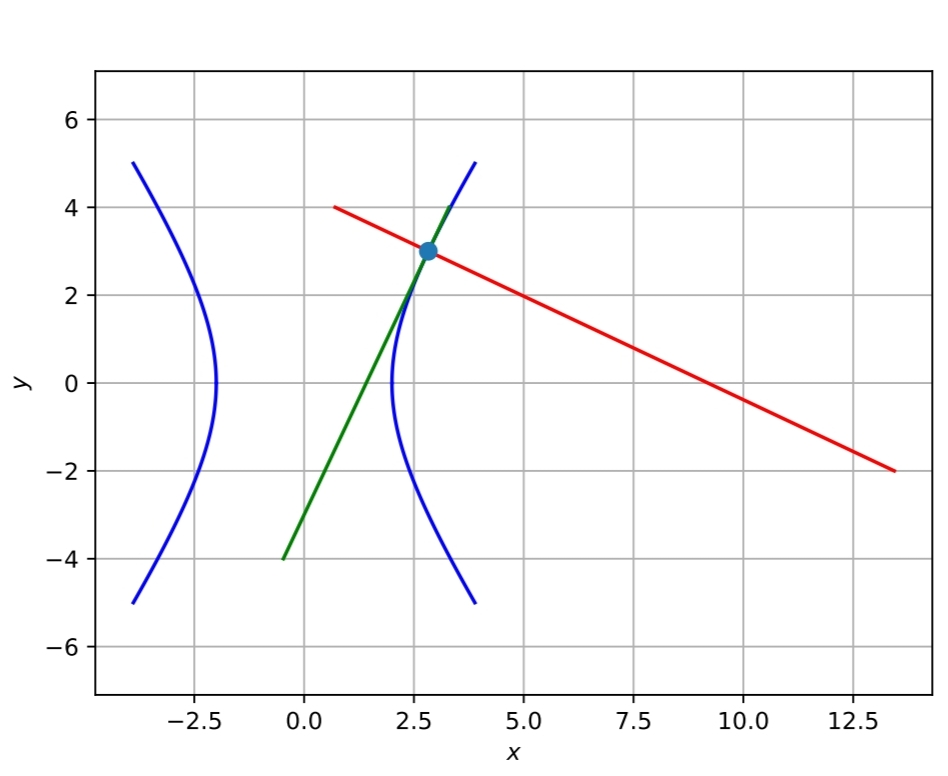
\includegraphics[scale=0.2]{main.jpg}}\vspace{2mm}\\
\centering{Figure}\vspace{2mm}\\
\centering \large\textsc{3  C}\footnotesize\textsc{ONSTRUCTION}\vspace{5mm}\\
\raggedright\large{The hyperbol is constructed with } 
\begin{center}
    \label{tab:truthtable}
    \setlength{\arrayrulewidth}{0.2mm}
\setlength{\tabcolsep}{5pt}
\renewcommand{\arraystretch}{1.25}
    \begin{tabular}{|c|c|c|}
    \hline % <-- Alignments: 1st column left, 2nd middle and 3rd right, with vertical lines in between
      \large\textbf{Symbol} & \large\textbf{Co-ordinates} & \large\textbf{Description}\\
      \hline
	    \large P & $\ \begin{pmatrix} 2\sqrt{2} \\ 3 \end{pmatrix}$ & \makecell {point on the \\ hyperbola} \\

	\large a & 2 &\makecell {distance from \\ the  vertex to \\ the center}\\
	\large b & 3 &\makecell {distance perpendicular \\ to the transverse axis \\ from the vertex to \\ the asymptote lines }\\
      \hline
   \end{tabular}
 \end{center}
\raggedright\large{The figure above is generated using python code provided in the below source code link.} \\
\begin{mdframed}
\raggedright\large{https://github.com/sivagayathri \\ /FWC/blob/main/matrices/conic/conic.py}
\end{mdframed}
\end{multicols}
\end{document}
